\documentclass[runningheads]{llncs}
\usepackage{graphicx}
\usepackage[utf8]{inputenc}
\usepackage[spanish]{babel}

\usepackage{Sweave}
\begin{document}
\Sconcordance{concordance:abstract.tex:abstract.Rnw:%
1 5 1 1 0 27 1 1 37 16 1 1 2 1 0 3 1 3 0 1 2 3 1 1 2 1 0 1 10 13 0 1 2 %
8 1}


\title{metR - An R package for meteorological fields}

%\titlerunning{Abbreviated paper title}
% If the paper title is too long for the running head, you can set
% an abbreviated paper title here
%
\author{Elio Campitelli\inst{1}}

%
\authorrunning{E. Campitelli}
% First names are abbreviated in the running head.
% If there are more than two authors, 'et al.' is used.
%
\institute{Centro de Investigaciones del Mar y la Atmósfera \\
    \email{eliocampitelli@cima.fcen.uba.ar}\\
    %\url{http://www.springer.com/gp/computer-science/lncs}
    }
%
\maketitle              % typeset the header of the contribution
%
% \begin{abstract}
\keywords{meteorología  \and data \and Another keyword.}
% \end{abstract}




\section{Introducción}


Gran parte de la investigación en ciencias de la atmósfera consiste en el análisis y visualización de datos.

Un software de visualización de datos meteorológicos y oceanográficos muy utilizado es GrADs (Grid Analysis and Display System) el cual permite leer y graficar campos escalares y vectoriales con gran facilidad. Sin emabrgo, su lenguaje de scripting es muy limitado, carece de capacidades estadísticas nativas y no existen gran cantidad de extensiones que las implementen. R, en cambio, posee implementaciones de virtualmente cualquier tratamiento estadístico usado en ciencias de la atmósfera y el paquete \texttt{raster} que permite leer y graficar datos geográficos con relativa facilidad, pero por su naturaleza los datos quedan opacados detrás de una estructura complicada que no es fácil hacer interactuar con otros paquetes; en particular, no es posible graficar utilizando \texttt{ggplot2}. 

La finalidad de \texttt{metR} es proveer facilidades en la lectura, manejo y visualización de datos meteorológicos en R utilizando estructuras comunes soportadas por la mayoría de los paquetes, de manera de poder beneficiarse de los aportes de la comunidad. Hace fuerte uso de `data.table` por su eficiencia en memoria y velocidad dada la gran cantidad de datos que suelen usarse en meteorología, y en \texttt{ggplot2} por su flexibilidad y facilidad en la creación de gráficos. 

\section{Ejemplo}

Como ejemplo, se usan los datos de altura geopotencial media mensual en el nivel de 700hPa entre 1990 y 2000, que vienen incluidos en `metR`. 

Se calculan las anomalías temporales para cada puntos de grilla y calcular el campo asociado a la primera componente principal para cada mes. Finalmente, se calcula el viento geostrófico correspondiente a ese campo. Todo este proceso toma unas pocas líneas de código y se integra sin esfuerzo en el \emph{workflow} de \texttt{data.table}. 

\begin{Schunk}
\begin{Sinput}
> geopotential[, gh.t := Anomaly(gh), by = .(lon, lat, month(date))]
> geopotential[, gh.t.w := gh.t*sqrt(cos(lat*pi/180))]
> eof <- geopotential[, EOF(gh.t.w ~ date | lon + lat, n = 1)$right, by = .(month(date))]
> eof[, c("u", "v") := GeostrophicWind(gh.t.w, lon, lat), by = .(month)]
\end{Sinput}
\end{Schunk}


Luego, se grafica el campo de geopotencial con contornos llenos de manera que haya una relación uno a uno entre los niveles graficados y los señalados en la escala de colores. El campo de movimiento, por su parte, se grafica con líneas de corriente. 

\begin{Schunk}
\begin{Sinput}
> binwidth <- 0.01
> ggplot(eof[month %in% 1], aes(lon, lat)) +
+    geom_contour_fill(aes(z = gh.t.w), circular = "x", 
+                      breaks = AnchorBreaks(0, binwidth, 0)) +
+    geom_streamline(aes(dx = dlon(u, lat), dy = dlat(v)), L = 30, 
+                    skip = 2) +
+    scale_fill_divergent(breaks = AnchorBreaks(0, binwidth, 0), 
+                         guide = "colorstrip", name = "") +
+    scale_y_latitude(ticks = 15) + scale_x_longitude() + geom_map +
+    coord_quickmap(xlim = c(0, 360), ylim = c(-90, -20)) +
+    theme_minimal() + theme_field()
\end{Sinput}
\end{Schunk}
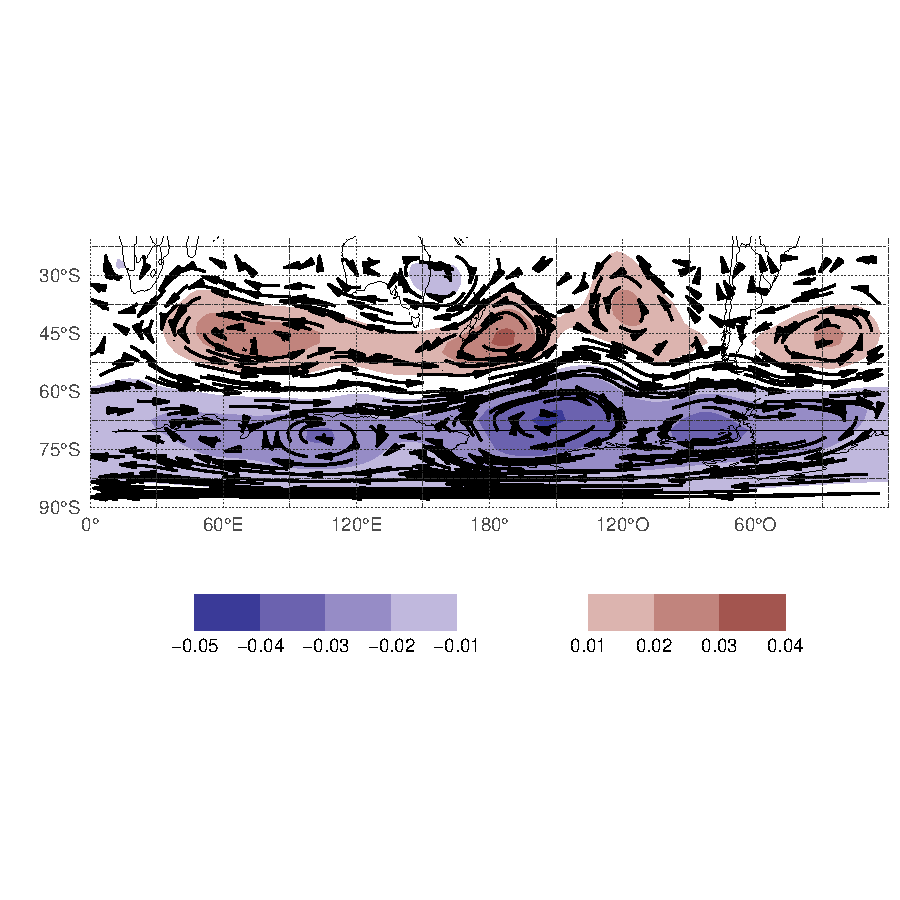
\includegraphics{abstract-example-plot}

\section{Limitaciones}

El uso de `data.table`s para el manejo de datos implica una importante limitación para \texttt{metR}. Muchas aplicaciones meteorológicas hacen uso de cantidades de datos que resultan imposibles cargar en memoria RAM en la mayoría de las computadoras personales. \texttt{metR} tampoco puede manejar campos que no se encuentren en en grillas regulares o en grillas proyectadas. En ambos casos paquetes como \texttt{raster} y \texttt{rasterVis} son indispensables. 

\texttt{metR} está en estado experimental y de activo desarrollo, tanto en crecimiento de funcionalidad como en refinamiento de interfaces y corrección de errores. Como todo proyecto de código abierto, es deseable además que a medida que sea adoptado por la comunidad, surgan nuevos casos de uso que incentiven su evolución más allá de las necesidades personales de un sólo desarrollador. 


\end{document}
